% resultados.tex
\chapter{Resultados}
\thispagestyle{fancy}

Como resultado deste trabalho, é apresentada uma ferramenta construida para operar junto ao Scrapy. Essa ferramenta utiliza o código do template em XML/WPT como entrada e produz o respectivo spider na linguagem Python, que utiliza o framework Scrapy como base para cumprir os objetivos de extração de informações estruturadas na Web.

\hyphenation{ou-tros}

A ferramenta aqui apresentada ainda encontra-se em desenvolvimento. Por ser uma contribuição ao Scrapy, um \textit{framework} de código aberto, esse protótipo poderá ser desenvolvido por outros membros da comunidade. O código-fonte desse protótipo encontra-se num repositório do Github (\texttt{http://github.com/}) disponível em \texttt{http://github.com/herberthamaral/}, no \emph{branch} "crawling-template".

Por não se tratar de uma ferramenta estável, o código originado do presente trabalho ainda não foi incorporado na linha de desenvolvimento principal do Scrapy, mas espera-se que isso seja feito em breve.

Apesar de ser um projeto de código aberto e disponibilizado publicamente, ainda não há contribuições de outros desenvolvedores. Um dos motivos é a proposital falta de divulgação: espera-se ter uma versão que possa ser considerada estável antes de apresentar esse projeto formalmente à comunidade.

Um dos aspectos positivos da abordagem adotada é que a ferramenta desenvolvida gera o código de spiders na linguagem de programação Python a partir de código em XML, permitindo que o programador faça altarações no código gerado, caso seja necessário. 

Como este trabalho não contempla, tampouco pretende contemplar, todas as facetas da criação de sistemas de recuperação de informações estruturadas na Web, a possibilidade do programador alterar o código gerado pode vir a ser bem útil em situações mais específicas. Por isso o objetivo deste trabalho é \emph{gerar código} ao invés de \emph{interpretar código} com o intuito de criar sistemas de recuperação de informações.

Pelo fato dos objetivos deste trabalho se basearem na criação de uma ferramenta que facilite a criação de sistemas de recuperação de informação na Web, duas análises podem ser feitas com os resultados: uma quantitativa e outra qualitativa. Quantitativa para mostrar as visíveis economias no processo de escrita/manutenção de código. Qualitativa para mostrar como os resultados obtidos podem levar a uma maior produtividade, menor curva de aprendizado e resultados mais rápidos. Também se faz necessária a demonstração de exemplos de sistemas de recuperação de informações reais criados a partir do uso da abordagem desenvolvida neste trabalho, bem como as dificuldades encontras e trabalhos futuros.

\section{Avaliação quantitativa}

A avaliação de sucesso no cumprimento dos objetivos deste projeto pode ser meramente subjetiva. Porém, há alguns critérios quantitativos ou subjetivos que podem ser discutidos, como a economia em linhas de código. 

A avaliação quantitativa leva em conta o número de linhas no formato XML/WPT necessárias para gerar o código em Python com o uso da ferramenta desenvolvida neste trabalho e é mensurada através da comparação do número de linhas de código, em ambas linguagens, necessárias para obter o mesmo resultado. Uma avaliação positiva é dada se o número de linhas de código gerado em Python for superior ao número de linhas utilizadas para escrever o template em XML.

Como exemplo, há o template mostrado na Listagem \ref{wpt_exemplo}.

\lstset{language=XML,
basicstyle=\scriptsize,
caption={Exemplo de template em WPT},
captionpos=b
}
\begin{lstlisting}[label=wpt_exemplo]
  <ow:wpt xmlns:ow="http://www.omfica.org/schemas/ow/0.9"
            ow:host="http://example.com">
  <ow:template ow:name="Template Example" ow:url="http://www.example.com/index.php">
      <ow:block ow:tagid="ex1" name="ex1"></ow:block>
  </ow:template> 
  </ow:wpt>
\end{lstlisting}

Com o uso da ferramenta desenvolvida neste trabalho, o template anterior corresponde ao código gerado em Python mostrado na Listagem \ref{spider_python_wpt_exemplo}.

\lstset{language=Python,
basicstyle=\scriptsize,
caption={\emph{Spider} gerado a partir do arquivo de entrada apresentado na listagem \ref{wpt_exemplo}},
captionpos=b
}
\begin{lstlisting}[label=spider_python_wpt_exemplo]
from scrapy.item import Item, Field

class TemplateExampleItem1(Item):
    ex1 = Field()

from scrapy.spider import BaseSpider
from scrapy.contrib.loader import XPathItemLoader

class TemplateExample(BaseSpider):
    name = 'example.com'
    allowed_domains = ['example.com']
    start_urls = [
        'http://www.example.com/index.php',
    ]
    
    def parse(self, response):
        l = XPathItemLoader(item = TemplateExampleItem1(),response=response)
        l.add_xpath('bubble','id("ex1")/text()') 
        i = l.load_item()
        yield i
\end{lstlisting}

O código em Python possui 20 linhas, 16 sem as linhas em branco, ao passo que o template possui apenas 5 linhas de código. Nesse exemplo, na pior das hipóteses, a economia de código gira em torno de 2/3 do original. A diferença fica mais evidente em um exemplo mais completo, como o mostrado na listagem \ref{wpt_exemplo_mais_completo}.

\lstset{language=XML,
basicstyle=\scriptsize,
caption={Exemplo mais completo de template em WPT},
captionpos=b
}
\begin{lstlisting}[label=wpt_exemplo_mais_completo]
<ow:wpt xmlns:ow="http://www.omfica.org/schemas/ow/0.9"
ow:host="http://example.com">
<ow:template ow:name="Template Example" ow:url="http://www.example.com/index.php">
  <ow:block ow:tagid="ex1" name="ex1"></ow:block>
  <ow:block ow:xpath="/html/body/p/text()" name="paragraph"></ow:block>
  
  <ow:block ow:xpath="/html/body/ul/li" name="menu">
    <ow:block ow:xpath="//a/text()" name="item" ow:type="repeatable"></ow:block>
    <ow:block ow:xpath="//a[@href]" name="url" ow:type="repeatable"></ow:block>
  </ow:block>
  
  <ow:block ow:xpath="/html/body/div[2]/ul/li" name="paginate">
    <ow:block ow:xpath="//a[@href]" name="url" ow:type="follow"></ow:block> <!-- follow -->
  </ow:block>
</ow:template> 
</ow:wpt>
\end{lstlisting}

Com o auxílio da ferramenta citada anteriormente, o código anterior em XML é utilizado para gerar código em Python mostrado na Listagem \ref{spider_python_wpt_exemplo_mais_completo}.

\lstset{language=Python,
basicstyle=\scriptsize,
caption={\emph{Spider} gerado a partir do arquivo de entrada apresentado na listagem \ref{wpt_exemplo_mais_completo}},
captionpos=b
}
\begin{lstlisting}[label=spider_python_wpt_exemplo_mais_completo]
from scrapy.item import Item, Field

class TemplateExampleItem1(Item):
    ex1 = Field()

class TemplateExampleItem2(Item):
    paragraph = Field()
    
class MenuItem(Item):
    item = Field()
    url = Field()
    
class Paginate(Item):
    url = Field()

from scrapy.spider import BaseSpider
from scrapy.contrib.loader import XPathItemLoader
from scrapy.selector import HtmlXPathSelector
from scrapy.http import Request

class TemplateExample(BaseSpider):
    name = 'example.com'
    allowed_domains = ['example.com']
    start_urls = [
        'http://www.example.com/index.php',
    ]

    def parse(self, response):
        l = XPathItemLoader(item = TemplateExampleItem1(),response=response)
        l.add_xpath('bubble','id("ex1")/text()') 
        i = l.load_item()
        yield i
        
        l = XPathItemLoader(item = TemplateExampleItem2(),response=response)
        l.add_xpath('paragraph','/html/body/p/text()') 
        i = l.load_item()
        yield i
        
        hxs = HtmlXPathSelector(response)
        for item in hxs.select('/html/body/ul/li'):
            l = XPathItemLoader(item = MenuItem(), selector=item)
            l.add_xpath('item','//li/a/text()') 
            l.add_xpath('url','//li/a[@href]') 
            i = l.load_item()
            yield i

        hxs = HtmlXPathSelector(response)
        for item in hxs.select('/html/body/div[2]/ul/li'):
            l = XPathItemLoader(item = Paginate(), selector=item)
            l.add_xpath('url','//li/a[@href]') 
            i = l.load_item()
            yield Request(item=i['url'],callback=self.parse)
            yield i
\end{lstlisting}

Neste segundo exemplo, o arquivo XML possui 15 linhas, ao passo que o código gerado possui cerca de 60 linhas, sendo aproximadamente 4 vezes menor.

\pagebreak
\section{Avaliação qualitativa}

Em uma comparação qualitativa, pode-se citar alguns critérios:

\begin{enumerate}
	\item Linguagens de propósito geral \emph{versus} \glspl{DomainSpecificLanguage}.
	\item Ganho de produtividade.
	\item Facilidade para o usuário final.
	\item Automação de processos.
\end{enumerate}

Linguagens de propósito geral servem para a construção de mais diversos tipos de sistemas, ao passo que linguagens de propósito específico são projetadas para resolver problemas em um domínio específico. Há um \emph{tradeoff} entre as duas abordagens: enquanto as linguagens de propósito geral são mais completas, elas também são mais complexas se comparadas com as linguagens de propósito específico para a mesma categoria de problema.

Quando se deixa de usar uma linguagem de propósito geral (Python) para utilizar outra de propósito específico (XML/WPT) o ganho de produtividade estará em eliminar preocupações não inerentes ao domínio. Com menos recursos e preocupações a serem considerados, o trabalho do usuário final é facilitado.

Por exemplo, quando se trabalha com uma linguagem de propósito geral (como Python, C/C++ ou Java), o programador dispõe de uma maior flexibilidade, pois o mesmo pode valer de estruturas de controle, repetição, variáveis, funções ou métodos, classes, objetos, interação com o sistema de arquivos e E/S, interação com outros sistemas e tratamento de exceções para desenvolver suas soluções. Além de todos os itens relacionados à linguagem de programação, o programador precisa ter domínio de técnicas de extração de informações de páginas na Web, em que, nos casos mais simples, envolve o conhecimento de uma linguagem de marcação (HTML, por exemplo), bibliotecas utilizadas para \emph{parsing} e bibliotecas para comunicação com servidores HTTP (\emph{HyperText Transfer Protocol} - Protocolo de Transferência de HiperTexto). No caso de uma linguagem específica de domínio baseada em XML, o programador precisará ter as mesmas noções de extração de informações de páginas na Web, porém sem a complexidade de lidar com uma linguagem de propósito geral e todas as suas respectivas dependências (bibliotecas), limitando-se apenas a conhecer a sintaxe do XML e as regras inerentes ao WPT.

O uso de XML pode trazer várias vantagens para a criação de sistemas de recuperação de informação. A principal é que qualquer linguagem de programação que dê suporte à XML pode criar templates. Como o trabalho de \emph{não} escrever código é sempre menor do que escrever \emph{algum} código, os usuários podem se beneficiar com a criação de sistemas que geram templates automaticamente. Por exemplo, um \emph{plugin} de um navegador Web pode permitir que o usuário selecione as seções de uma determinada página que gostaria que fossem recuperadas automaticamente e então gerar o template correspondente. 

Uma outra vantagem do uso de XML como meio para geração desses sistemas é a baixa dependência de uma única linguagem de programação, como a linguagem Python utilizada neste trabalho, uma vez que qualquer outra linguagem com as devidas bibliotecas pode interpretar XML e gerar código para qualquer outra linguagem de programação. Com isso, há como diminuir o nível de acoplamento entre a solução desenvolvida e a linguagem utilizada, de forma que todo o código em XML possa ser reaproveitado para geração de outros sistemas em outras linguagens de programação sem maiores problemas.

\pagebreak
\section{Exemplos reais}

Para fornecer melhores bases de entendimento deste trabalho, a seguir são apresentadas exemplos de casos de uso da ferramenta desenvolvida em conjunto com todo o processo de identificação de elementos na página e escrita do template.

\subsection{Exemplo 1 - Página de editais do Ministério da Cultura}

A página de editais do Ministério da Cultura, que se encontra em \url{http://www.cultura.gov.br/site/categoria/editais-ministerio-da-cultura/}, contém a lista dos últimos editais publicados, com seus respectivos títulos, categorias e informações gerais, como demonstrado na figura \ref{minc}.

\begin{figure} [ht]
	\centering
	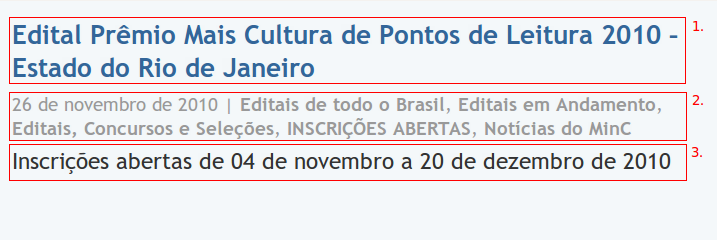
\includegraphics[scale=0.8]{minc.png}
	\caption{Seleção dos elementos que compõem uma chamada de notícia de edital}
	\label{minc}
\end{figure}

A seguir, as legendas das respectivas áreas destacadas:

\begin{enumerate}
	\item Título da notícia
	\item Metadados (data e tags)
	\item Mais informações
\end{enumerate}

Analisando o código HTML da seleção, obtém-se os seguintes seletores \gls{xpath}:

\begin{itemize}
	\item \textbf{Base} - \texttt{/html/body/div[2]/div[1]/ol[1]/li}
	\item \textbf{Título} - \texttt{//h3/a/text()}
	\item \textbf{Metadados} - \texttt{//p/text()}
	\item \textbf{Mais informações} - \texttt{//div/p/text()}
\end{itemize}

Como os itens desejados (chamadas de notícias) se repetem na página, é necessário indicar qual será o padrão de repetição, o que nesse caso é indicado pelo seletor \textbf{Base}: todos os itens de lista (\texttt{li}) que se encontram em \texttt{/html/body/div[2]/div[1]/ol[1]}. Os demais seletores derivam de cada item da lista indicada por \textbf{Base}.

Seguindo as especificações do Website Parse Template (WPT), o template necessário para obter a lista de editais com seus respetivos atributos se encontra na listagem \ref{wpt_minc}.

\lstset{language=XML,
basicstyle=\scriptsize,
caption={Template utilizado para recuperar os editais do sítio do Ministério da Cultura},
captionpos=b
}
\begin{lstlisting}[label=wpt_minc]
<ow:wpt xmlns:ow="http://www.omfica.org/schemas/ow/0.9"
 ow:host="http://example.com">
<ow:template ow:name="minc_news" 
 ow:url="http://www.cultura.gov.br/site/categoria/editais-ministerio-da-cultura/">
  <ow:block ow:xpath="/html/body/div[2]/div[1]/ol[1]/li" name="lista_news" ow:type="repeatable">
    <ow:block ow:xpath="//h3/a/text()" name="titulo" ></ow:block>
    <ow:block ow:xpath="//p/text()" name="meta"></ow:block>
    <ow:block ow:xpath="//div/p/text()" name="mais_info"></ow:block>
  </ow:block>
</ow:template> 
</ow:wpt>
\end{lstlisting}

O template apresentado na Listagem \ref{wpt_minc} reflete nas regras definidas anteriormente, com o bloco \texttt{lista\_news} como seletor dos itens de lista onde ficam as chamadas dos editais e contendo três blocos: o \texttt{titlulo}, o \texttt{meta} e o \texttt{mais\_info}, que representam as informações de cada chamada edital. Tendo salvo o template anterior num arquivo chamado \texttt{minc.xml}, o comando \texttt{scrapy importwpt minc.xml} exibe a saída mostrada na listagem \ref{python_wpt_minc}.

\pagebreak
\lstset{language=Python,
basicstyle=\scriptsize,
caption={Código gerado pela ferramenta desenvolvida utilizando o arquivo \texttt{minc.xml} da listagem \ref{wpt_minc} como entrada},
captionpos=b
}
\begin{lstlisting}[label=python_wpt_minc]
from scrapy.item import Item, Field

class minc_newsItem1(Item):
    lista_news = Field()
    titulo = Field()
    meta = Field()
    mais_info = Field()


from scrapy.spider import BaseSpider
from scrapy.contrib.loader import XPathItemLoader

class minc_news(BaseSpider):
    name = 'www.cultura.gov.br'
    allowed_domains = ['www.cultura.gov.br']
    start_urls = ['http://www.cultura.gov.br/site/categoria/editais-ministerio-da-cultura/']

    def parse(self, response):
        
        hxs = HtmlXPathSelector(response)
        for item in hxs.select('/html/body/div[2]/div[1]/ol[1]/li'):
            l = XPathItemLoader(item = minc_newsItem2(), selector=item)
            l.add_xpath('titulo','//h3/a/text()')
            l.add_xpath('meta','//p/text()')
            l.add_xpath('mais_info','//div/p/text()')

            i = l.load_item()
            yield i

\end{lstlisting}


O spider demonstrado na listagem \ref{python_wpt_minc} pode ser executado com o comando \texttt{scrapy runspider /caminho/para/minc.py} e produz a saída (devidamente adaptada para uma melhor visualização em folhas de papel A4) mostrada na listagem \ref{scrapy_wpt_minc}

\lstset{basicstyle=\scriptsize,
caption={Saída produzida pela execução do scraper da listagem \ref{python_wpt_minc}},
captionpos=b
}
\begin{lstlisting}[label=scrapy_wpt_minc]
scrapy runspider testescrapy/spiders/minc.py
2010-12-02 07:49:31-0200 [scrapy] INFO: Scrapy 0.11.0 started (bot: testescrapy)
2010-12-02 07:49:31-0200 [scrapy] DEBUG: Enabled extensions: TelnetConsole, SpiderContext, 
WebService, CoreStats, MemoryUsage, CloseSpider
															  
2010-12-02 07:49:31-0200 [scrapy] DEBUG: Enabled scheduler middlewares: DuplicatesFilterMiddleware

2010-12-02 07:49:31-0200 [scrapy] DEBUG: Enabled downloader middlewares: HttpAuthMiddleware, 
DownloadTimeoutMiddleware, UserAgentMiddleware, RetryMiddleware, DefaultHeadersMiddleware, 
RedirectMiddleware, CookiesMiddleware, HttpCompressionMiddleware, DownloaderStats

2010-12-02 07:49:31-0200 [scrapy] DEBUG: Enabled spider middlewares: HttpErrorMiddleware, 
OffsiteMiddleware, RefererMiddleware, UrlLengthMiddleware, DepthMiddleware
																     
2010-12-02 07:49:31-0200 [scrapy] DEBUG: Enabled item pipelines: 
2010-12-02 07:49:31-0200 [scrapy] DEBUG: Telnet console listening on 0.0.0.0:6023
2010-12-02 07:49:31-0200 [scrapy] DEBUG: Web service listening on 0.0.0.0:6080
2010-12-02 07:49:31-0200 [www.cultura.gov.br] INFO: Spider opened
2010-12-02 07:49:32-0200 [www.cultura.gov.br] DEBUG: Crawled (200) 
<GET http://www.cultura.gov.br/site/categoria/editais-ministerio-da-cultura/> (referer: None)
Item recuperado: <titulo=Divulgada lista dos convocados para oficina presencial de Florianopolis> 

Item recuperado: <titulo=Premio Hip Hop> 

Item recuperado: <titulo=Edital Ideias Criativas para 20 de novembro de 2010 - 
						 Dia Nacional da Consciencia Negra> 

Item recuperado: <titulo=Edital do Programa de Apoio a Traducao de Autores Brasileiros> 

Item recuperado: <titulo=Premio Luso-Brasileiro de Dramaturgia Antonio Jose da Silva - 2010> 

Item recuperado: <titulo=Premio Mais Cultura Pontos de Leitura do estado do Ceara> 

Item recuperado: <titulo=Programa de Intercambio e Difusao Cultural - Edital numero 1/2010> 

Item recuperado: <titulo=Edital de Pontos de Leitura de Sao Leopoldo> 

Item recuperado: <titulo=Premio Mais Cultura de Apoio as Bibliotecas Comunitarias do Estado do Ceara> 

Item recuperado: <titulo=Edital 22 Anos da Palmares> 

Item recuperado: <titulo=Premio Mais Cultura de Pontinhos de Cultura de Fortaleza 2010> 

Item recuperado: <titulo=Premio Mais Cultura de Pontos de Leitura de Fortaleza> 

2010-12-02 07:49:32-0200 [www.cultura.gov.br] INFO: Closing spider (finished)
2010-12-02 07:49:32-0200 [www.cultura.gov.br] INFO: Spider closed (finished)
\end{lstlisting}


\subsection{Exemplo 2 - Obtendo as últimas perguntas no \textit{StackOverflow}}

O \textit{StackOverflow}\footnote{\url{http://stackoverflow.com/}} é um sítio gratuito de perguntas e respostas sobre programação \cite{stackoverflow}. O objetivo deste exemplo é recuperar as últimas perguntas feitas com alguns de seus respectivos dados: resumo da pergunta, usuário que a fez, número de visualizações, número de votos e número de respostas.

A página em questão (\url{http://stackoverflow.com/about}) contém um índice com últimas perguntas feitas em que cada índice possui a estrutura descrita na Figura \ref{stackoverflow}.

\begin{figure} [ht]
	\centering
	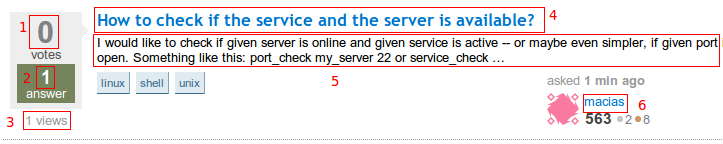
\includegraphics[scale=0.8]{stackoverflow.png}
	\caption{Seleção dos elementos que compõem um item da lista de perguntas do StackOverflow}
	\label{stackoverflow}
\end{figure}

A seguir, as legendas das respectivas áreas destacadas:

\begin{enumerate}
	\item Número de votos
	\item Número de respostas
	\item Número de visualizações
	\item Título da pergunta
	\item Resumo da pergunta
	\item Nome do usuário que fez a pergunta
\end{enumerate}

Analisando o código HTML da seleção, obtém-se os seguintes seletores \gls{xpath}:

\begin{itemize}
	\item \textbf{Base} - \texttt{//div[@id='questions']/div}
	\item \textbf{Titulo} - \texttt{//div[@class='summary']/h3/a/text()}
	\item \textbf{Resumo} - \texttt{//div[@class='summary']/div[1]/text()}
	\item \textbf{Usuário} - \texttt{//div[@class='summary']/div[3]/div[3]/a/text()}
	\item \textbf{Vizualizações} - \texttt{//div[@class='statscontainer']/div[@class='views']/text()}
	\item \textbf{Votos} - \texttt{//div[1]/div[2]/div[1]/div[@class='votes']/span/strong/text()}
	\item \textbf{Respostas} - \texttt{//div[1]/div[2]/div[2]/strong/text()}
\end{itemize}

O item \textbf{Base} indica a base de repetição da lista de perguntas da página. Dentro do container \textbf{Base} encontra-mse os outros elementos que compõe o item a ser recuperado. O WPT equivalente às seleções anteriores é descrito na listagem \ref{wpt_stackoverflow}.

\lstset{language=XML,
basicstyle=\scriptsize,
caption={Template utilizado para recuperar as últimas perguntas do sítio do StackOverflow},
captionpos=b
}
\begin{lstlisting}[label=wpt_stackoverflow]
<ow:wpt xmlns:ow="http://www.omfica.org/schemas/ow/0.9"
    ow:host="http://stackoverflow.com">
      
    <ow:template ow:name="stackoverflow" 
        ow:url="http://stackoverflow.com/questions">
       
        <ow:block ow:xpath="//div[@id='questions']/div" name="questions" ow:type="repeatable"> 
            <ow:block ow:xpath="//div[@class='summary']/h3/a/text()" name="tiulo" >
            </ow:block>
            
            <ow:block ow:xpath="//div[@class='summary']/div[1]/text()" name="resumo"> 
            </ow:block>
            
            <ow:block ow:xpath="//div[@class='summary']/div[3]/div[3]/a/text()" name="usuario" >
            </ow:block>

            <ow:block ow:xpath="//div[@class='statscontainer']/div[@class='views']/text()" 
                name="views" ></ow:block>

            <ow:block ow:xpath="//div[1]/div[2]/div[1]/div[@class='votes']/span/strong/text()" 
                name="votes" >
            </ow:block>

            <ow:block ow:xpath="//div[1]/div[2]/div[2]/strong/text()" name="answers" >
            </ow:block>
        </ow:block>
              
     </ow:template> 

</ow:wpt>
\end{lstlisting}

Tendo salvo o conteúdo descrito na listagem \ref{wpt_stackoverflow} no arquivo \texttt{stackoverflow.xml}, o comando para gerar o respectivo código em Python é \texttt{scrapy importwpt stackoverflow.xml}. O código gerado é mostrado na listagem \ref{py_stackoverflow}.

\lstset{language=XML,
basicstyle=\scriptsize,
caption={Template utilizado para recuperar os editais do sítio do Ministério da Cultura},
captionpos=b
}
\begin{lstlisting}[label=py_stackoverflow]

from scrapy.item import Item, Field

class stackoverflowItem1(Item):
    questions = Field()
    tiulo = Field()
    resumo = Field()
    usuario = Field()
    views = Field()
    votes = Field()
    answers = Field()


from scrapy.spider import BaseSpider
from scrapy.contrib.loader import XPathItemLoader
from scrapy.selector import HtmlXPathSelector
from scrapy.http import Request

class stackoverflow(BaseSpider):
    name = 'stackoverflow.com'
    allowed_domains = ['stackoverflow.com']
    start_urls = ['http://stackoverflow.com/questions']

    def parse(self, response):
        
        hxs = HtmlXPathSelector(response)
        for item in hxs.select('//div[@id="questions"]/div'):
            l = XPathItemLoader(item = stackoverflowItem1(), selector=item)
            l.add_xpath('tiulo','//div[@class="summary"]/h3/a/text()')
            l.add_xpath('resumo','//div[@class="summary"]/div[1]/text()')
            l.add_xpath('usuario','//div[@class="summary"]/div[3]/div[3]/a/text()')
            l.add_xpath('views','//div[@class="statscontainer"]/div[@class="views"]/text()')
            l.add_xpath('votes','//div[1]/div[2]/div[1]/div[@class="votes"]/span/strong/text()')
            l.add_xpath('answers','//div[1]/div[2]/div[2]/strong/text()')

            i = l.load_item()
            yield i
\end{lstlisting}

A Listagem \ref{out_stack} mostra uma saída adaptada da execução do spider descrito na Listagem \ref{py_stackoverflow}.

\begin{lstlisting}[label=out_stack]
2010-12-04 21:04:17-0200 [scrapy] INFO: Scrapy 0.11.0 started (bot: testescrapy)
2010-12-04 21:04:17-0200 [scrapy] DEBUG: Enabled extensions: TelnetConsole, 
SpiderContext, WebService, CoreStats, MemoryUsage, CloseSpider

2010-12-04 21:04:17-0200 [scrapy] DEBUG: Enabled scheduler middlewares: DuplicatesFilterMiddleware
2010-12-04 21:04:17-0200 [scrapy] DEBUG: Enabled downloader middlewares: HttpAuthMiddleware, 
  DownloadTimeoutMiddleware, UserAgentMiddleware, RetryMiddleware, DefaultHeadersMiddleware, 
  RedirectMiddleware, CookiesMiddleware, HttpCompressionMiddleware, DownloaderStats
  
2010-12-04 21:04:17-0200 [scrapy] DEBUG: Enabled spider middlewares: HttpErrorMiddleware, 
OffsiteMiddleware, RefererMiddleware, UrlLengthMiddleware, DepthMiddleware
2010-12-04 21:04:17-0200 [scrapy] DEBUG: Enabled item pipelines: 
2010-12-04 21:04:17-0200 [scrapy] DEBUG: Telnet console listening on 0.0.0.0:6023
2010-12-04 21:04:17-0200 [scrapy] DEBUG: Web service listening on 0.0.0.0:6080
2010-12-04 21:04:17-0200 [stackoverflow.com] INFO: Spider opened
2010-12-04 21:04:23-0200 [stackoverflow.com] DEBUG: Crawled (200) 
    <GET http://stackoverflow.com/questions> (referer: None)
    
Item recuperado <titulo=C# - sorting a list inside of a struct,usuario=Tyler>
Item recuperado <titulo=JavaScript - Smooth Movement / Resizing,usuario=jSherz>
Item recuperado <titulo=C++ Linker Errors,usuario=Yelnats>
Item recuperado <titulo=How can I access my trackpad in C#?,usuario=Serg>
Item recuperado <titulo=(English, Perl, Python, Ruby) comparison on a code 
  fragment-by-fragment basis?,usuario=blunders>
Item recuperado <titulo=MySQL 5.1 Memory Table ,usuario=James>
Item recuperado <titulo=How to access the file which is in Production Server 
  from a class in a Jar,usuario=kumar>

Item recuperado <titulo=Does anyone know where I can find some good WebGl 
  documentation?,usuario=Catalin Dumitru>
  
Item recuperado <titulo=Scaml syntax highlighting on Emacs,usuario=alp247>
Item recuperado <titulo=Cx_freeze - How can I Install the shared libraries 
  to /usr/lib,usuario=MetaDark>
  
Item recuperado <titulo=PHP random string generator,usuario=ssen>
Item recuperado <titulo=How do I use Watir::Waiter::wait_until to force
  Chrome to wait?,usuario=karim79>
Item recuperado <titulo=React differently if second time user visits domain,
  usuario=Mike Grace>
  
Item recuperado <titulo=return flat text from .net webservice ? ,usuario=user391179>
Item recuperado <titulo=General Questions about Entity Framework 
  vs. Enterprise Library & a few others,usuario=icode.cs>
  
2010-12-04 21:04:23-0200 [stackoverflow.com] INFO: Closing spider (finished)
2010-12-04 21:04:23-0200 [stackoverflow.com] INFO: Spider closed (finished)
\end{lstlisting}

%----------------%<---------------------



\pagebreak
\chapter{Considerações Finais}
\thispagestyle{fancy}

\section{Dificuldades encontradas}

Apesar da abundante documentação e mesmo não possuindo uma má qualidade de código ou baixa cobertura de testes, uma das principais dificuldades foi aderir à arquitetura e estilo de codificação do Scrapy para que a padronização entre componentes fosse mantida.

O framework em si possui um tamanho considerável (759 arquivos em 13/11/2010 \footnote{Informação obtida através do comando \texttt{find | wc -l} }), portanto, leva-se um tempo para acostumar-se com a estrutura de diretórios, arquivos e padrões de nome.

Não foi possível encontrar referências acadêmicas do Scrapy, um dos motivos pelos quais somente a respectiva documentação oficial foi utilizada.

O formato WPT possui apenas informações sobre a disposição dos elementos em uma página e seus respectivos significados (ontologia). Tal fato leva ao incoveniente de haver diferentes \emph{schemas} XML em um mesmo arquivo para determinar outras informações, como nome dos variáveis do código gerado e formato de persistência dos dados obtidos.

Ainda não é possível o uso de WPT para determinar o verbo HTTP a ser utilizado. Atualmente, todas as requisições feitas com os spiders gerados a partir do WPT são feitas através do HTTP GET, não sendo possível utilizar outros verbos HTTP como POST, PUT, DELETE e PATCH. 

As regras de validação formam outra dificuldade relacionada ao WPT: verificação de validade de URLs, caminhos XPATH, validação de templates, blocos e nomes de elementos. Como a validação ocorre em vários elementos e o XML é um formato hierárquico, validações recursivas precisaram ser feitas, e, dependendo do nível de recursão, tratamentos especiais teriam que ser dados. Como um exemplo, considere o trecho de código da listagem \ref{problemas_wpt_blocos1}:

\lstset{language=XML,
basicstyle=\scriptsize,
caption={Hierarquia de blocos planos e de um nível},
captionpos=b
}
\begin{lstlisting}[label=problemas_wpt_blocos1]
 ...
  <ow:block ow:xpath="/bloco1" name="raiz">
    <ow:block ow:xpath="//caminho/para/um" name="raiz_um"></ow:block>
    <ow:block ow:xpath="//caminho/para/dois" ow:type="repeatable" name="raiz_dois"></ow:block>
  </ow:block>
 
  <ow:block ow:xpath="/bloco2" name="dois"></ow:block>
  ...
\end{lstlisting}

O bloco com nome \texttt{dois} é um bloco de nível único e o bloco com nome \texttt{raiz} é um bloco hierárquico com um nível. Os blocos de nível único são fáceis de serem interpretados pois representam apenas um item na página a ser obtido. Já os blocos com um nível formam itens compostos por um ou mais elementos de nível único. Blocos com o atributo \emph{ow:type="repeatable"} (como o bloco de nome \texttt{raiz\_dois}) em um contexto que nem todos são repetíveis precisam de um tratamento especial. Blocos de nível único repetíveis são tratados de maneira similar.

O principal problema acontece quando há um bloco com um nível maior que um, como o mostrado na listagem \ref{problemas_wpt_blocos2}. Este tipo de caso ainda não é tratado pela ferramenta, por ainda ser complexo de lidar. De fato, ainda não há uma solução definitiva para blocos com mais de um nível, pois todas as regras anteriores, incluindo verificação de nomes e verificação de blocos com repetições, devem ser aplicadas.

\lstset{language=XML,
basicstyle=\scriptsize,
caption={Hierarquia de blocos de dois níveis},
captionpos=b
}
\begin{lstlisting}[label=problemas_wpt_blocos2]
 ...
  <ow:block ow:xpath="/bloco_raiz" name="raiz">

    <ow:block ow:xpath="//caminho/para/um" name="um">
    	<ow:block ow:xpath="//caminho/para/um_pt_um" name="um_pt_um"></ow:block>
    	<ow:block ow:xpath="//caminho/para/um_pt_dois" name="um_pt_dois"></ow:block>
    </ow:block>
    
    <ow:block ow:xpath="//caminho/para/dois" name="dois"></ow:block>
    <ow:block ow:xpath="//caminho/para/tres" name="tres"></ow:block>
    
  </ow:block>
  ...
\end{lstlisting}

Questões como "quantos níveis poderão ser suportados?", "como os blocos do nível N deverão ser tratados?","qual a profundidade máxima de níveis que a ferramenta poderá suportar?", "como blocos repetíveis serão tratados em cada nível", "como ficará a questão da navegação em outras páginas a partir de links para serem seguidos forem detectados em blocos de níveis mais inferiores?" ainda permanecem sem resposta, devido à natureza e complexidade de achar a resposta das mesmas.

Há ainda a preocupação com a qualidade e legibilidade do código gerados, uma vez que a ferramenta desenvolvida não visa substituir o programador, mas sim auxilia-lo. A ferramenta precisa gerar código devidamente organizado e com alguns comentários para melhor orientação. A indentação obrigatória da linguagem Python é uma característica que ajuda neste quesito, porém não deixa de causar problemas com relação a indentação na geração de código.

A biblioteca padrão para testes disponíveis no Python 2.6 (utilizado neste trabalho), a \texttt{unittest}, não possui um método de comparação de strings linha-a-linha, que é uma funcionalidade útil quando se trata testes de métodos que geram código. Isso significa que, se um texto precisa ser comparado com outro em um teste unitário, os dois serão comparados em sua totalidade, não linha-a-linha, o que dificulta os testes dos métodos responsáveis por geração de código.

Esta dificuldade torna os testes de geração de código mais trabalhosos, pois é necessário observar cada caractere com cautela quando os dois textos, o esperado e o obtido, falham no teste unitário.

Outra dificuldade encontrada nos testes unitários foi o teste de comandos, devido ao tempo que os testes levam para serem executados. A suíte de testes do Scrapy levam aproximadamente 30 segundos para serem executados\footnote{Os testes são executados com o comando \texttt{bin/runtests.sh scrapy.tests} dentro do diretório raiz do código fonte do Scrapy }, o que atrasa o desenvolvimento, já que a cada modificação no código, os testes precisam ser executados.
\vfill

\pagebreak
\section{Trabalhos futuros}

O atual sistema ainda possui algumas limitações, como a falta de persistência dos dados obtidos. No atual cenário, é necessário que o programador altere o código fonte gerado para que os itens gerados pelo Scrapy durante a recuperação de informações sejam persistidos em disco.

O presente trabalho conseguiu atingir o objetivo de facilitar a criação e manutenção de sistemas de recuperação estruturada na Web, porém é possível facilitar ainda mais este trabalho. Plugins para navegadores Web podem ser criados de forma que os usuários possam criar os Website Parse Templates (WPT) através de uma interface visual.

Como o significado dos dados obtidos (metadados) não fazem parte deste trabalho, a seção \texttt{<ow:ontology>} do WPT é deliberadamente ignorada. Em trabalhos futuros, é provável que a mesma seja utilizada e então o protótipo aqui criado terá de ser modificado. 

\emph{Plugins} como o Firebug \cite{firebug} para o navegador Mozilla Firefox permitem inspecionar a estrutura do conteúdo de sítios na Wieb. Com ele, é possível selecionar elementos, mudar estilos e conteúdo, analisar o tráfego utilizado pelo acesso ao sítio e \emph{debugar} JavaScript. Usando o Firebug como plataforma, é possível desenvolver um outro complemento que facilite a criação de Htmltemplates, o que poderia facilitar ainda mais o trabalho de criação de sistemas de recuperção de informações na Web.
